\documentclass[t]{beamer} 
\usepackage{amsmath}
\usepackage{amsthm}
\usepackage[T1]{fontenc}
\usepackage{lmodern}
\usepackage{color}
\usepackage{xcolor}
\usepackage{hyperref}
\usepackage{multirow,varwidth} % used for SL table
\usepackage{tikz}
\usepackage{multicol}
\usepackage{graphicx}
\usepackage{etoolbox}
\usepackage{bm}
\usepackage[abs]{overpic}
\usepackage{pict2e}
\usepackage{animate}
\usepackage{verbatim}
\usepackage{soul}
\usepackage{xmpmulti}
\usepackage{subfig}
\usepackage{media9}
\usepackage{tabularx, booktabs}


\usetheme{PaloAlto}
\usecolortheme{seahorse}


\newenvironment{withoutheadline}{ 
\setlength{\headheight}{0pt} 
\setbeamertemplate{headline}{}}

\setbeamercolor*{block title example}{fg=white,
bg= black!30!blue}
\setbeamercolor*{block body example}{fg=black,
bg= blue!5}

\setbeamertemplate{frametitle continuation}{}

\setbeamertemplate{footline}{}

\setbeamertemplate{itemize items}[circle]
\setbeamertemplate{navigation symbols}[only frame symbol]
\setbeamerfont{framesubtitle}{size=\large}
\newcommand{\nl}{\newline}
\newcommand{\pl}{\parallel}
\newcommand{\openr}{\hbox{${\rm I\kern-.2em R}$}}
\newcommand{\openn}{\hbox{${\rm I\kern-.2em N}$}}
\newcommand{\argmax}[1]{\underset{#1}{\operatorname{argmax}}\;} 
\newcommand{\argmin}[1]{\underset{#1}{\operatorname{argmin}}\;} 

%\title{{\bf Super-Efficient Estimation of Average Treatment Effect based on Randomized Controlled Trial Augmented with External Controls or Observational Study}}
\title{{\bf Adaptive TMLE for Estimation of Average Treatment Effect based on Randomized Controlled Trial Augmented with External RWD}}
%\subtitle{Application to robust integration of RCT with External Observational Study}
\author{Mark van der Laan}


%\institute{Jiann-Ping Hsu/Karl E. Peace Professor in Biostatistics \& StatisticsUniversity of California, Berkeley}

\date{October 28-29, 2024, Workshop Statistical Methods for Hybrid RCT using RWD\\
\
{\tiny \vspace{5pt} Joint methodological work with Sky Qiu, Lars van der Laan\\
Adaptive TMLE:  Lars vanderLaan et al. (2023), https://arxiv.org/abs/2307.12544\newline
RCT+RWD A-TMLE: upcoming article for special issue. Collaboration joint with NN-group.
}
}

\begin{document}

\begin{frame}[noframenumbering]
\titlepage
\end{frame}

%\section{Goal}\begin{frame}{General Estimation Problem}\begin{itemize}\item We observe $n$ i.i.d. copies of $O\sim P_0\in {\cal M}$ for a realistic statistical model ${\cal M}$.\item Let $\Psi:{\cal M}\rightarrow\mathcal{R}$ be a pathwise differentiable  target parameter of interest with canonical gradient $D^*_P$ at $P$. $\pl D^*_P\pl_{\infty}<M$ for some $M<\infty$.\item Statistical estimand: $\Psi(P_0)$.\item Construct a good finite sample robust estimator of $\Psi(P_0)$.\item In particular, in situations in which Cramer-Rao lower bound $\mbox{VAR}D^*_P(O)$ is so large that it does not correspond with a reasonable finite sample bias variance trade-off  (e.g., lack of positivity).\end{itemize}\end{frame}\section{Efficient TMLE}\begin{frame}{Efficient TMLE (vdL, Rubin, 2006)}\begin{itemize}\item Construct initial estimator ${\bf P}_n$; determine a least favorable path $\{{\bf P}_{n,\epsilon}:\epsilon\in (-\delta,\delta)\}\subset {\cal M}$ through ${\bf P}_n$ with score $D^*_{{\bf P}_n}$ at $\epsilon =0$.\item Compute MLE $\epsilon_n =\arg\max_{\epsilon}P_n L({\bf P}_{n,\epsilon})$, where $L(P)$ is a valid loss function so that $\Psi(\arg\min_P P_0L(P))=\Psi(P_0)$.\item Let ${\bf P}_n^*={\bf P}_{n,\epsilon_n}$. The TMLE is given by $\Psi({\bf P}_n^*)$.\item By construction, $\Psi({\bf P}_n^*)-\Psi(P_0)=(P_n-P_0)D^*_{{\bf P}_n^*}+R({\bf P}_n^*,P_0)$, with $R(P,P_0)\equiv \Psi(P)-\Psi(P_0)-(P-P_0)D^*_P$ an exact second order remainder. \item Using the Highly Adaptive Lasso as initial estimator ${\bf P}_n$, we are guaranteed that $\Psi({\bf P}_n^*)$ is asymptotically efficient estimator of $\Psi(P_0)$ (van der Laan, 2017).\end{itemize}\end{frame}\section{Regularizing TMLE}\begin{frame}{Finite sample robust TMLE}\begin{itemize}\item The current literature on TMLE has proposed various modifications of TMLE that regularize the TMLE to be better behaved in finite samples when the support is limited.\item For example, in censored and causal inference literature: collaborative TMLE, outcome-adaptive TMLE, super-efficient TMLE.\item These proposed regularizations have in common that they all concern targeted estimation of the orthogonal nuisance function $g(P_0)$ that is needed in targeting step, while $\Psi(P_0)=\Psi_1(Q_0)$ only depends on certain factors of likelihood. \item Typically, these variations preserve asymptotic efficiency but adapt the targeting step towards the data to carefully trade-off bias reduction with variance gain.\end{itemize}\end{frame}\begin{frame}\begin{itemize}\item Finite sample simulations, theoretical results such as collaborative double robustness etc, have shown that these regularizations are crucial for robust finite sample behavior for poorly supported parameters. \item However, we never developed a truly unifying approach (and super-efficiency theory)!\item Fortunately, Lars did: Lars van der Laan et al. (2023), Adaptive debiased machine learning.\end{itemize}\end{frame}


%\section{Limitations of effciency}\begin{frame}{Limitations of Efficient Estimators such as TMLE}\begin{itemize}\item Due to lack of nonparametric support, if ${\cal M}$ is close to nonparametric, then $D^*_{P_0}(o)$ can have very large values. \item In that case, confidence intervals for standard TMLE will be wide and no significant finding can be obtained.\item However if we would use plug-in HAL $\Psi({\bf P}_n)$ (possibly super-efficient) we might very well still find a significant true result. Somehow, the targeting step can blow up a good initial estimator.\item This is due to an efficient estimator to be regular along all paths through $P_0$, including paths that appear to be contradicting the data. \end{itemize}\end{frame}

%\begin{frame}{An efficient estimator cannot adapt to structure in the true data distribution}\begin{itemize}\item For example, suppose $O=(W,A,Y)$ and $\Psi(P)=E_PE_P(Y\mid A=1,W)$. A plug-in HAL might end up fitting an additive model for the regression $E(Y\mid A,W)$ that contains the true regression.\item An efficient estimator of $\Psi(P_0)$ for this additive model would be well supported and have reasonable variance. \item But an efficient estimator for a nonparametric model protects itself against any kind of fluctuation of the data distribution, and as a consequence carries out a bias reduction that ({\bf asymptotically}) holds up uniform in $P$ in a ball around $P_0$.\item In other words, it needs to remain asympotically unbiased under fluctuations adding a 100 way interaction.\end{itemize}\end{frame}

\section{Motivating example}
\begin{frame}{Integrating RCT with Observational Data}\begin{itemize}\item Suppose we observe data on two studies indicated by $S\in \{0,1\}$: $(S_i,W_i,A_i,Y_i)$, $i=1,\ldots,n$. 
\item In study $S=1$, treatment is randomized (RCT), so that the ATE can be robustly estimated.
\item Study $S=0$ is an external RWD study. 
\item  We make no other assumptions on likelihood beyond possible knowledge of $g(A\mid S,W)$.
\item However, the RCT is underpowered due to small control arm or small overall sample size.\item Therefore, a TMLE of the ATE based on $S=1$ only would have large confidence intervals lacking power at reasonable alternatives. \item Can we utilize the external study $S=0$ from the real world to obtain a more efficient estimator of the ATE?  Without adding assumptions!
\end{itemize}
\end{frame}
\begin{frame}
\begin{itemize}
\item Dang et al (2023) developed an ES-CV-TMLE. Rejects RWD if biased relative to RCT.
\item Here, we develop an Adaptive TMLE that learns bias in RWD and corrects pooled estimator.
%\item We revisit this example in detail later
\end{itemize}\end{frame}

\section{A-TMLE RCT$+$RWD}
\begin{frame}{Motivating example: oral semaglutide on cardiovascular outcomes (Dang et al. 2023)}
\small
\begin{itemize}
\item \textit{Causal question:} \textbf{risk of MACE within one year} if all patients in the target population were prescribed \textbf{oral semaglutide} plus standard-of-care compared to if all patients were prescribed \textbf{standard-of-care} alone?
\item \textit{Set up:} a single \textbf{RCT} (PIONEER 6) vs. a \textbf{hybrid} randomized-external data study.
\item \textit{Results:} 
\begin{itemize}
\item Under the single RCT: \\ \textbf{-1.30\% (95\% CI -2.60\%, 0.00\%)}. 
\item Under the hybrid design using ES-CVTMLE: \\ \textbf{-1.53\% (95\% CI -2.75\%, -0.30\%)}.
\end{itemize}
\item \textit{Conclusion}: importance of the \textbf{\textit{Causal Roadmap}}, using \textbf{RWD} to inform regulatory approval process, \textbf{power gain} of test for superiority, \textbf{reduced participation-time} without initiation of a GLP1-RA.
\end{itemize}
\end{frame}


%\begin{frame}{Lets reset benchmarks for our estimator}\begin{itemize}
%\item {\bf Super-efficient estimator:}Suppose that we require that our estimator of $\Psi(P_0)$ is asymptotically linear at any $P_0\in {\cal M}$, and regular along paths through $P_0$ that stay in an oracle model ${\cal M}_0\subset {\cal M}$, approximated by a data adaptive submodel ${\cal M}_n$ satisfying $P_0\in {\cal M}_0$.\item Then, we can construct ${\cal M}_0$-super-efficient estimators that still provide asymptotically valid confidence interval and are still robust under perturbations of $P_0$ that stay in the model ${\cal M}_0$. \item {\bf Regularized efficient estimator:} If our data adaptive model ${\cal M}_n$ approximates ${\cal M}_0={\cal M}$, let the estimator behave as an efficient estimator under model ${\cal M}_n$ that approximates the a-priori specified model ${\cal M}$ as sample size converges to infinity but in a way that carefully balances finite sample bias and variance.\end{itemize}\end{frame}


\section{A-TMLE of ATE}
\begin{frame}{Adaptive TMLE of ATE}
\begin{itemize}
\item Let $O=(W,A,Y)$; ${\cal M}$ nonparametric; $\Psi(P)=E_P\tau_P(W)$; $\tau_P=E_P(Y\mid A=1,W)-E_P(Y\mid A=0,W)$.
\item Consider loss function $L_{m_0,g_0}(\tau)$ indexed by nuisance parameters $m_0=E_0(Y\mid W)$ and $\bar{g}_0=P_0(A=1\mid W)$:
\[
L_{m,g}(\tau)=\left( Y-m(W)-(A-g(1\mid W))\tau\right)^2.\]
\item {\bf Double robust loss for CATE:} We have $\tau_0=\arg\min_{\tau}P_0 L_{m,g}(\tau)$ if $m=m_0$ or $g=g_0$. 
\end{itemize}
\end{frame}
\begin{frame}{Adaptive TMLE of ATE}
\begin{itemize}
\item Let $\sum_j\beta(j)\phi_j$ be a high dimensional linear combination of splines $\phi_j$ as in HAL. Define
\[
\beta_n=\arg\min_{\beta,\pl\beta\pl_1<C_n}P_n L_{m_n,g_n}\left(\sum_j \beta_j\phi_j\right).\]
Then, refit $\sum_{j,\beta_n(j)\not =0}\beta_j\phi_j$ unpenalized (relax-HAL). 
\item Let $\tau_n=\sum_j\beta_n(j)\phi_j$.  $\psi_n=P_n \tau_n$ is an adaptive TMLE  where the learned working model ${\cal M}_n$ for $P_0$ is the semiparametric regression model selected by HAL. 
\item It is super-efficient corresponding with oracle model ${\cal M}_0$ the limit of HAL-working model ${\cal M}_n$ ({\bf or just efficient if ${\cal M}_0={\cal M}$}).
\end{itemize}
\end{frame}
\section{A-TMLE RCT$+$RWD}

%\begin{frame}{Observed data and statistical model}\begin{itemize}\item $S\in\{0,1\},$ study indicator ($S=1$ denotes RCT, $S=0$ denotes RWD);\item $W$ patient characteristics;\item $A\in\{0,1\},$ binary treatment;\item $Y$ continuous outcome;\item Observe $n$ i.i.d $O=(S,W,A,Y)\sim P_0\in\mathcal{M}$.\item We factorize the density of $O$ as follows $$p(s,w,a,y)=p_S(s)p_W(w\mid s)g_A(a\mid s,w)q_Y(y\mid s,w,a).$$\item For the statistical model, we only make assumption on $g_A(a\mid s,w)$.end{itemize}\end{frame}
%\begin{frame}{Design considerations}\begin{itemize}\item If one matches external subjects with RCT subjects, one might approximately  have that $W\perp S$.\item If one samples externals from same population as the RCT, then $W\perp S$.\item If one has external controls and treated, and one matches external control with external treated, one might approximately have$A\perp W$, given $S=0$. \item Under such designs, both $p_W(W\mid S)$ and $g_A(A\mid S,W)$ are easily learned.\end{itemize}\end{frame}

\begin{frame}{Causal  and statistical estimand}
\begin{itemize}
\item RCT-ATE $\Psi^F_0=E_PE_P(Y_1-Y_0\mid S=1,W)$.
\item Due to $S=1$ being an RCT, we have $\Psi^F_0$ equals {\small
\[ \psi_0=E_0\left( E_0(Y\mid S=1,W,A=1)-E_0(Y\mid S=1,W,A=0)\right).\]}
\item Note in  outer expectation, we take the average over the \textcolor{red}{pooled covariate distribution}. 
\item \textit{Oral semaglutide case study}: What would the risk difference be \textbf{if all patients in the target population were enrolled} in the trial? The target population should \textbf{not} contain individuals with 0 probability of being enrolled in the trial. Factors to consider: inclusion/exclusion criteria of PIONEER 6, time-frame, patient characteristics, healthcare engagement, etc. (Dang et al. 2023)
\end{itemize}
%\small
%\begin{table}
%\centering
%\begin{tabular}{m{11cm}}
%\tableheadrow
%\tableheadcol{\textit{Context: oral semaglutide case study}}\\
%\textit{What would the risk difference be \textbf{if all patients in the target population were enrolled} in the trial? The target population should \textbf{not} contain individuals with 0 probability of being enrolled in the trial. Factors to consider: inclusion/exclusion criteria of PIONEER 6, time-frame, patient characteristics, healthcare engagement, etc. (Dang et al. 2023)}
%\end{tabular}
%\end{table}
\end{frame}
%\begin{frame}{Identification assumptions}\begin{itemize}\item Mean exchangeability in the trial \textcolor{red}{(true by design of RCT)}: $$\EE(Y_a\mid S=1,W,A=a)=\EE(Y_a\mid S=1,W), \ a\in\mathcal{A}$$\item Positivity of receiving treatment in the trial \textcolor{red}{(true by design of RCT)}: $$0<\PP(A=1\mid S=1,W)<1, \ P_W\text{-a.e.}$$\item Positivity of trial enrollment: $$\PP(S=1\mid W)>0, \ P_W\text{-a.e.}$$\end{itemize}\end{frame}

%\begin{frame}{Statistical estimand}\begin{itemize}\small\item RCT-ATE: $$\Psi(P_0)=\EE[\EE(Y\mid S=1,W,A=1)-\EE(Y\mid S=1,W,A=0)]$$\item Note, for the outer expectation, we take the average over the \textcolor{red}{pooled covariate distribution}. That is, we average over $p_W=p_{W\mid S=0}p_{S=0}+p_{W\mid S=1}p_{S=1}.$\end{itemize}\end{frame}
\begin{frame}{Decomposition of the target estimand as difference  pooled-ATE and bias term (Dang et al. 2023)}
%\small\begin{itemize}
%\item Target estimand, \textbf{RCT-ATE} estimand: $\Psi(P_0)=E_0E_0(Y\mid S=1,W,A=1)-E_0E_0(Y\mid S=1,W,A=0)]$.\item 1st component, \textbf{pooled-ATE} estimand: $\tilde{\Psi}(P_0)=E_0\tau_0(W)$, where$\tau_0=E_0(Y\mid W,A=1)-E_0(Y\mid W,A=0)$.\item 2nd component, \textbf{bias} estimand: \[\Psi^\#(P_0)=\tilde{\Psi}(P_0)-\Psi(P_0),\]so that\[ \Psi(P_0)=\tilde{\Psi}(P_0)-\textcolor{red}{\Psi^\#(P_0)} \ \text{\textcolor{red}{bias correction}}\]\end{itemize}\end{frame}

%\begin{frame}{Pooled ATE and bias estimand}
\begin{itemize}
\item 1st component, \textbf{pooled-ATE} estimand: $\tilde{\Psi}(P)=E_P\tau_P(W)$.
\item 2nd component, \textbf{bias} estimand: $\Psi^\#(P)=\tilde{\Psi}(P)-\Psi(P)$:
$$\Psi^\#(P)=E_P[\Pi(0\mid W,0)\tau^S_P(W,0)-\Pi(0\mid W,1)\tau^S_P(W,1)],$$
 where $$\Pi(s\mid W,A)=P(S=s\mid W,A),$$ and \[\tau_P^S(W,A)=E_P(Y\mid S=1,W,A)-E_P(Y\mid S=0,W,A).\]
\item Thus
\[ \Psi(P_0)=\tilde{\Psi}(P_0)-\textcolor{red}{\Psi^\#(P_0)} \ \text{\textcolor{red}{bias correction}}.\]
\end{itemize}
\end{frame}

\begin{frame}{Adaptive-TMLE for bias estimand $\Psi^{\#}$}
\begin{itemize}
\item For pooled ATE $\tilde{\Psi}(P_0)$, we  could either use a regular TMLE of pooled ATE or the above A-TMLE.
%\item A nonparametric framework that combines \textbf{data-driven model selection} and debiased \textbf{machine learning} techniques to construct \textbf{asymptotically linear}, \textbf{adaptive}, and \textbf{super-efficient} estimators for pathwise differentiable functionals (van der Laan et al. 2023).
%\item We will apply it here to estimate the \textbf{pooled-ATE} and the \textbf{bias} estimands.
\item For the bias estimand $\Psi^{\#}(P_0)$, analogue to A-TMLE for ATE,  we will use relax-HAL to learn a \textbf{working submodel for the conditional effect $\tau^S_0$ of the study indicator} $S$ on the outcome $Y$ (implying a submodel ${\cal M}_n$). 
\item The corresponding A-TMLE of bias estimand also includes targeting an initial estimator $\Pi_n$ of $\Pi_0=P_0(S\mid W,A)$, and one estimates the expectation over $W$ with the empirical mean. 
\end{itemize}
\end{frame}

\begin{frame}{Benefits of using A-TMLE include}
\begin{itemize}
\item Nominal \textbf{type I error control} without extra assumptions.
\item Not only estimates the magnitude of the bias, also takes advantage of the \textbf{learn-able structure of the bias}. Allows \textbf{full utilization} of both RCT and RWD data, more gain in efficiency.
\item The bias working model \textbf{mitigates large variances} due to inverse-weighting, finite sample robust.
\end{itemize}
\end{frame}

%\begin{frame}{Double robustness for projection estimand}\begin{itemize}\item The TMLE and A-TMLE of the pooled ATE estimand $\tilde{\Psi}(P_0)$ are double robust. In particular, if $g(A\mid W,S=0)$ is correctly estimated, the TMLE will be valid.\item The A-TMLE of the bias parameter $\Psi^{\#}(P_0)$ is double robust so that it will be valid if $g(A\mid W,S=0)$ is correctly estimated. \item We also have a robustness w.r.t. misspecification of the HAL of the conditional effect of $S$ on $Y$, given $W,A$.\item What is precise statement?\end{itemize} \end{frame}
\section{Simulations}

\begin{frame}{Candidate estimators to compare}
\footnotesize
\begin{table}[]
\resizebox{\columnwidth}{!}{
\begin{tabular}{ m{1.5cm} m{8.5cm}}
\toprule
\multicolumn{1}{c}{\textbf{Estimator}} & \multicolumn{1}{c}{\textbf{Description}} \\
\midrule
A-TMLE & Our proposed estimator, applying the A-TMLE framework to estimate both the pooled-ATE $\tilde{\Psi}$ and the bias $\Psi^{\#}$. \\
\midrule
ES-CVTMLE & An estimator for integrating RCT with RWD within the TMLE framework, data-adaptively chooses between RCT-only or pooled-ATE to optimize bias-variance trade-off. (Dang et al. 2023) showed its superior efficiency gain over alternatives. \\
\midrule
PROCOVA & A prognostic score covariate-adjustment method (Schuler et al. 2022). \\
\midrule
TMLE & A standard TMLE for the target parameter. \\
\midrule
RCT-only & A standard TMLE for ATE parameter using RCT data alone, serving as the best estimator in the absence of external data.\\
\bottomrule
\end{tabular}
}
\end{table}
\end{frame}

\begin{frame}{Simulation 1: simple bias}
\centering
\vspace{1cm}
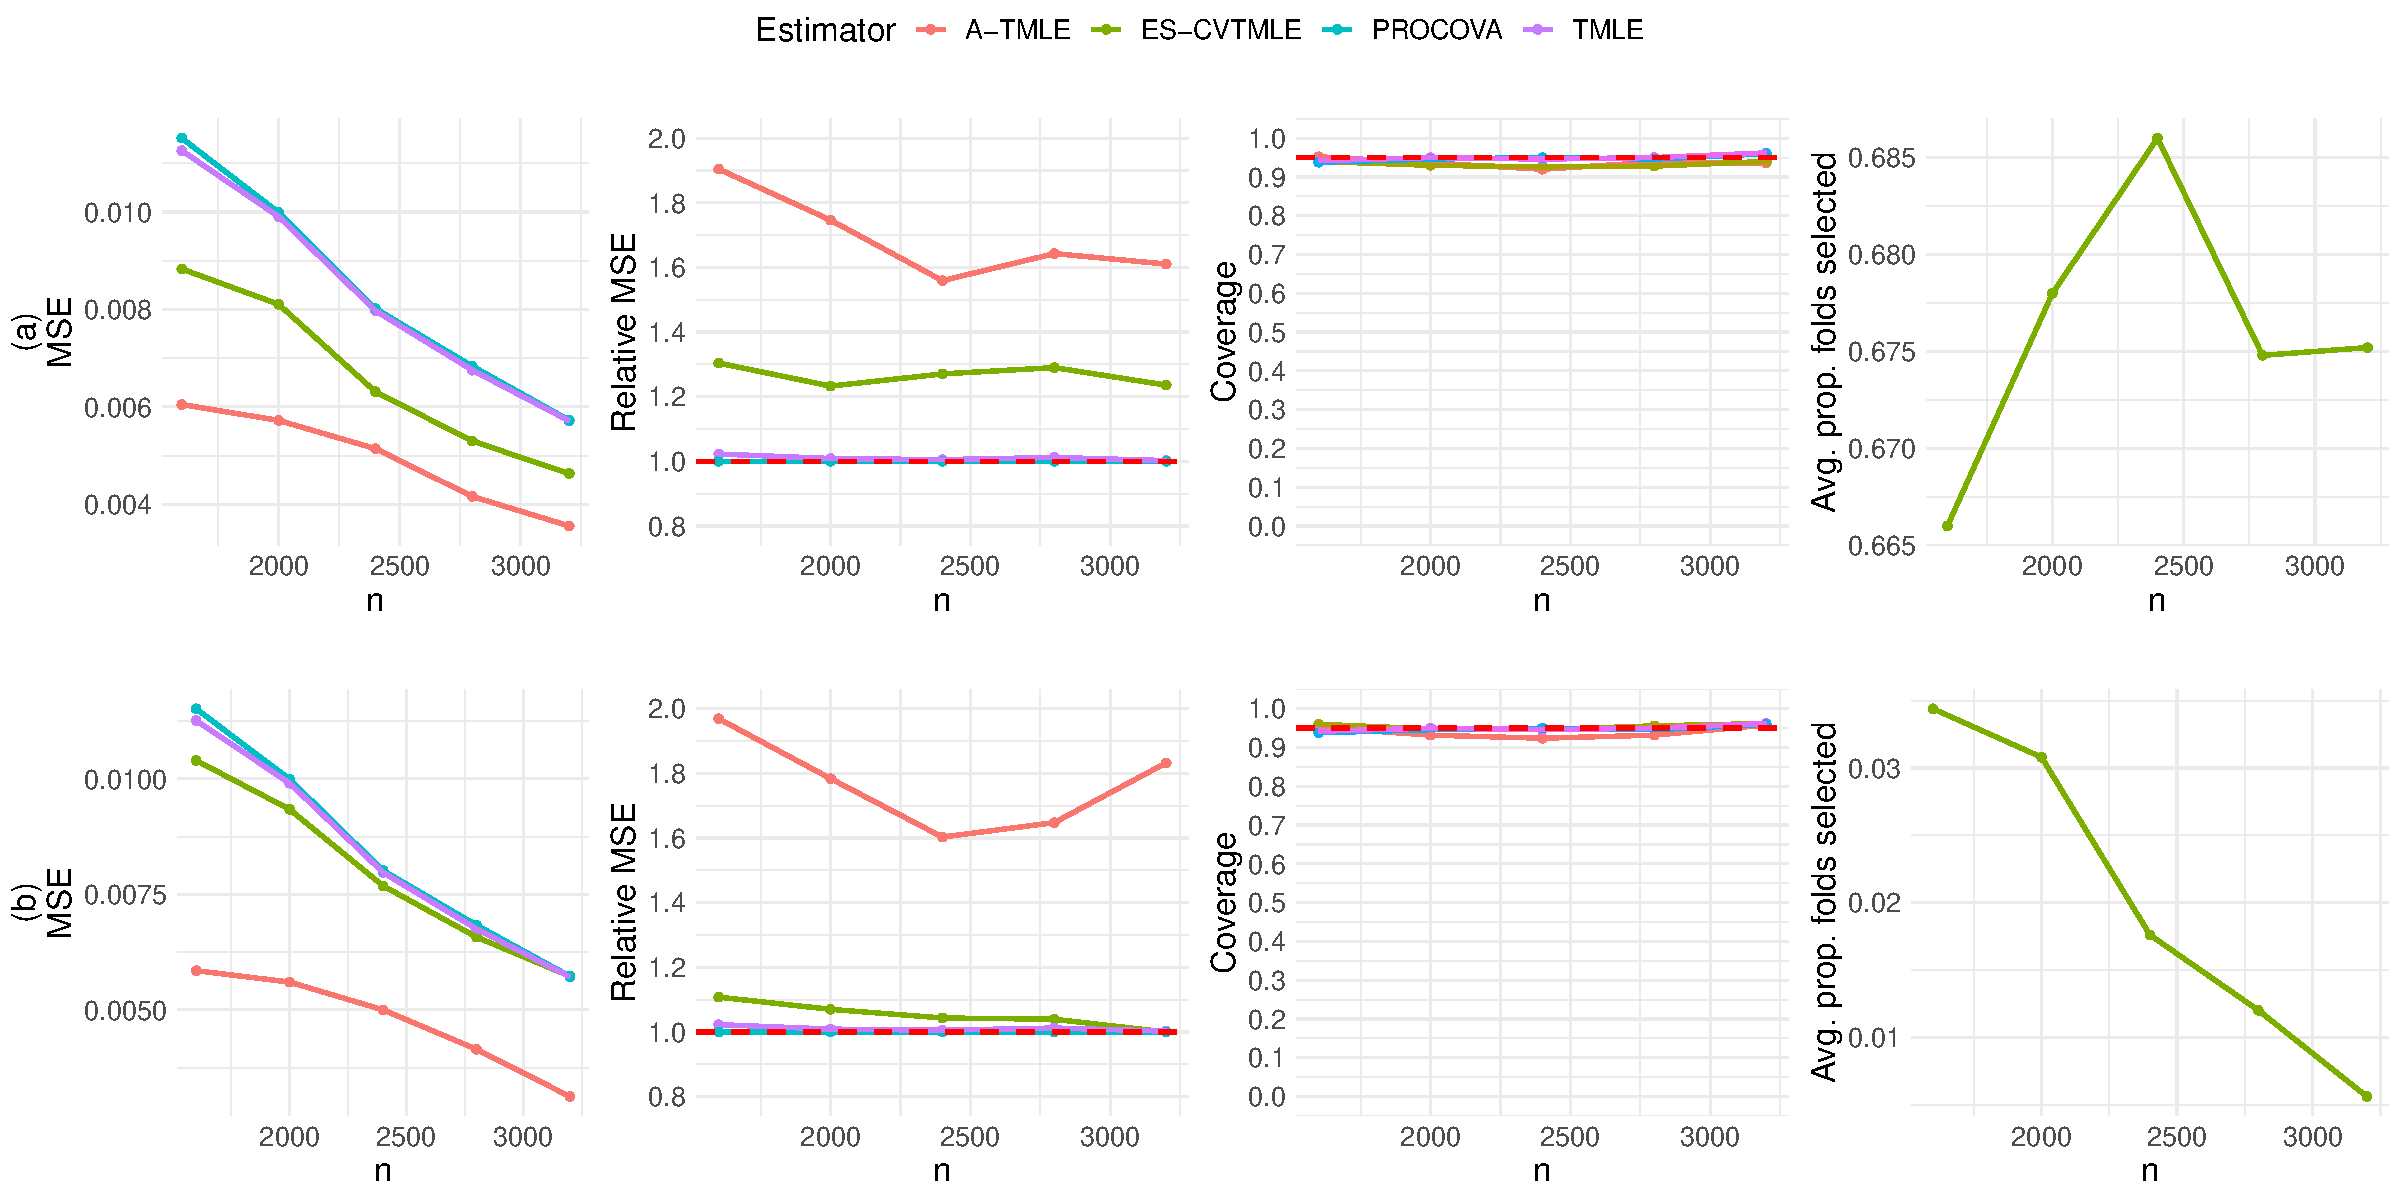
\includegraphics[width=1\textwidth,height=0.65\textheight]{simple.pdf}
\end{frame}

\begin{frame}{What if the bias is not a simple parametric form?}
\begin{itemize}
\item \textbf{Highly adaptive lasso (HAL)} is a maximum likelihood estimator over all (or subset of) \textit{càdlàg} functions (right continuous with left limits) with bounded variation norm (Benkeser and van der Laan 2016).
\item In our case, we can use HAL to data-adaptively learn the working submodel for conditional effect of the study indicator $S$.
\item Advantages of HAL: 
\begin{itemize}
\item It is \textbf{flexible} and can approximate almost all functions encountered in practice, without making any smoothness assumptions on the true functional form;
\item It \textbf{converges} to the true function at a \textbf{fast} rate $n^{-1/3}(\log n)^{2(d-1)/3}$;
\item It is an \textbf{MLE}.
\end{itemize}
\end{itemize}
\end{frame}

\begin{frame}{Simulation 2: complex bias}
\centering
\vspace{1cm}
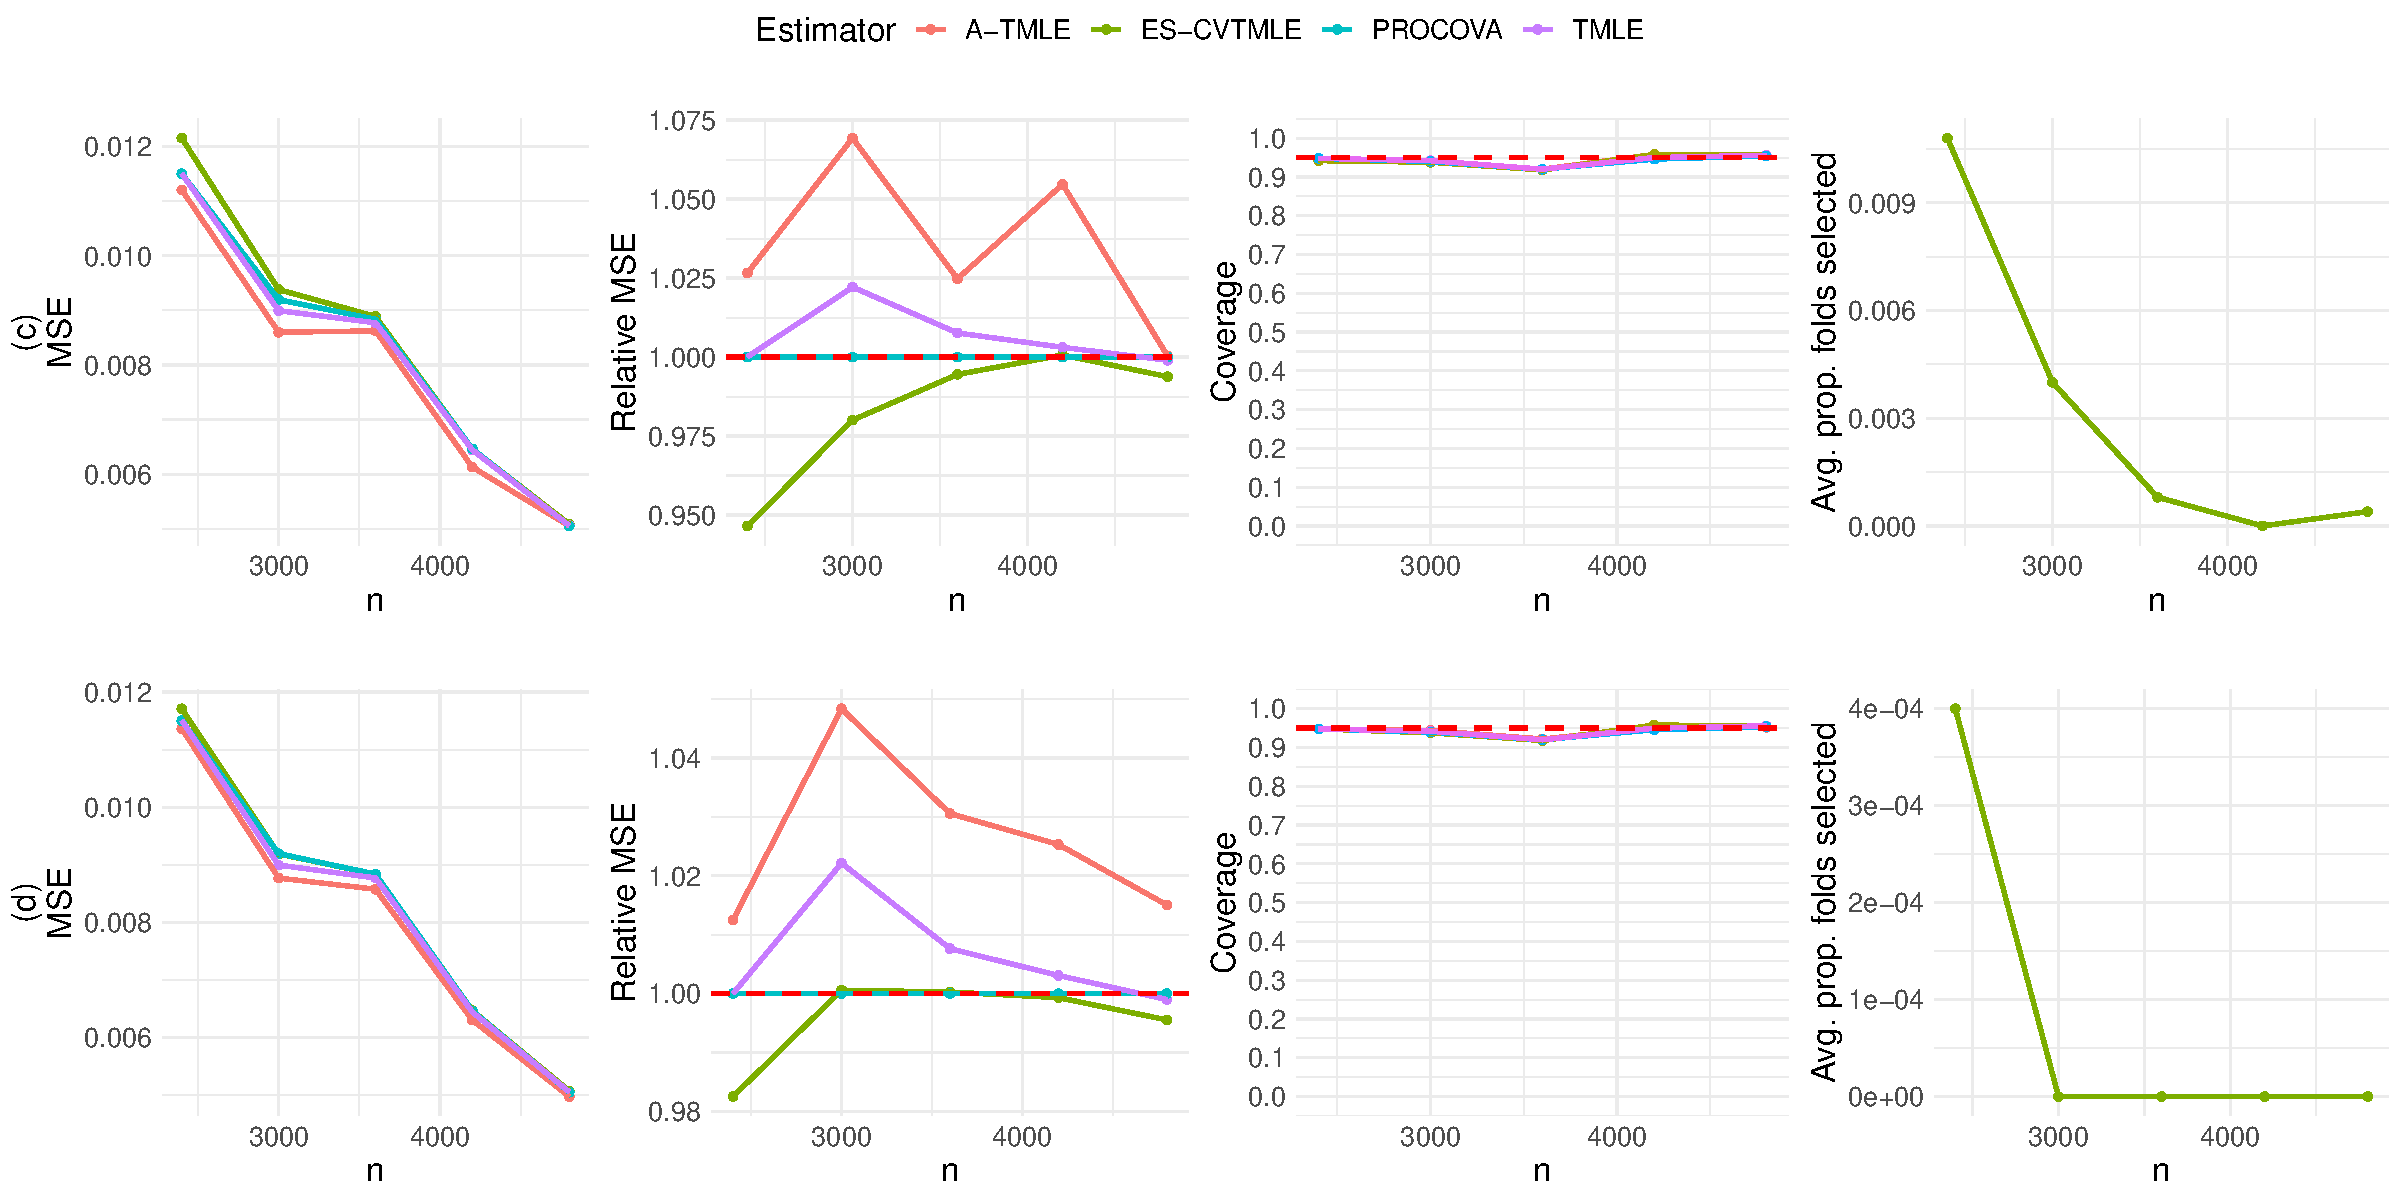
\includegraphics[width=1\textwidth,height=0.65\textheight]{complex.pdf}
\end{frame}

\begin{frame}{95\% CI width comparisons}
\begin{table}[ht]
\centering
\caption{A-TMLE's 95\% CI width as a percentage of other methods'.}
\label{tab:ci_width}
\resizebox{\columnwidth}{!}{
\begin{tabular}{ccccc}
\toprule
\textbf{Method} & \textbf{Scenario (a)} & \textbf{Scenario (b)} & \textbf{Scenario (c)} & \textbf{Scenario (d)} \\
\midrule
ES-CVTMLE & 66.1\% & 60.4\% & 98.3\% & 98.2\% \\
Regular TMLE & 59.1\% & 61.2\% & 99.1\% & 99.1\% \\
PROCOVA & 59.0\% & 61.1\% & 99.0\% & 99.0\% \\
RCT-only & 59.0\% & 61.1\% & 99.0\% & 99.0\% \\
\bottomrule
\end{tabular}
}
\end{table}
\end{frame}

%\begin{frame}{Simulation 1: super-efficiency}
%\begin{itemize}
%\item Combined data (sample size $n$) consists of:
%\begin{itemize}
%\item $\sim 20\%$ RCT patients, and
%\item $\sim 80\%$ RWD patients.
%\end{itemize}
%\item RWD has both \textbf{treated} and \textbf{control} patients.
%\item We consider 3 bias scenarios:
%\begin{itemize}
%\item No bias in RWD;
%\item Small bias (learn-able) in RWD;
%\item Large bias (learn-able) in RWD.
%\end{itemize}
%\end{itemize}
%\end{frame}

%\begin{frame}{Candidate estimators for comparison}
%\begin{itemize}
%\item A-TMLE
%\item ES-CVTMLE (Dang et al. 2023)
%\item TMLE (nonparametric, uses only RCT data for estimating outcome regression, but averages over pooled-covariate distribution; ``defines" the nonparametric efficiency bound)
%\end{itemize}
%\end{frame}

%\begin{frame}{}
%\centering
%\vspace{1.2cm}
%\includegraphics[width=1\textwidth,height=0.45\textheight]{mse.pdf}
%\end{frame}

%\begin{frame}{}
%\centering
%\vspace{1.2cm}
%\includegraphics[width=1\textwidth,height=0.45\textheight]{relative.pdf}
%\begin{itemize}
%\item Reference level: TMLE for the ATE that completely ignores RWD.
%\end{itemize}
%\end{frame}

%\begin{frame}{}
%\centering
%\vspace{1.2cm}
%\includegraphics[width=1\textwidth,height=0.45\textheight]{cover.pdf}
%\end{frame}

%\begin{frame}{Simulation 2: complex bias}
%\begin{itemize}
%\small
%\item \textbf{Bias is no longer learn-able by a main-term LASSO, we need to use HAL to approximate it.}
%\end{itemize}
%\end{frame}

%\begin{frame}{}
%\centering
%\vspace{1.2cm}
%\includegraphics[width=1\textwidth,height=0.45\textheight]{HAL_relative.pdf}
%\begin{itemize}
%\item Reference level: TMLE for the ATE that completely ignores RWD.
%\end{itemize}
%\end{frame}

%\begin{frame}{}
%\centering
%\vspace{1.2cm}
%\includegraphics[width=1\textwidth,height=0.45\textheight]{HAL_cover.pdf}
%\end{frame}

\begin{frame}{Lessons learned from simulations}
\footnotesize
\begin{table}[]
\resizebox{\columnwidth}{!}{
\begin{tabular}{p{3cm}p{3cm}p{3cm}}
\toprule
\textbf{Bias Type} & \textbf{Existing Methods} & \textbf{A-TMLE} \\
\midrule
No bias & Integrate external data, large efficiency gain & Bias working model is zero, \textbf{large}
efficiency gain \\
\midrule
Magnitude of the bias at the boundary of acceptance/rejection & Tend to be unstable & Learns bias, \textbf{large} efficiency gain \\
\midrule
Magnitude of the bias large & Reject external data, no efficiency gain & Learns bias, \textbf{large} efficiency gain \\
\midrule
Complex bias & Efficiency gain driven by bias magnitude & Working model adapts to the complexity
of the bias, \textbf{at least as efficient as an efficient estimator} that uses RCT data only \\
\bottomrule
\end{tabular}
}
\end{table}
\end{frame}


\begin{frame}{Double robustness: projection estimands}
\begin{itemize}
\item The pooled-ATE estimand $\tilde{\Psi}_{\mathcal{M}_{n,1}}(P_0)$ admits double robust estimation. If $g_0(1\mid W)\equiv P_0(A=1\mid W)$ is correctly specified, then the estimator remains unbiased regardless of estimations of $\tilde{\theta}_0(W)\equiv E_0(Y\mid W)$ or $\tilde{\tau}_0(W)\equiv E_0(Y\mid W,A=1)-E_0(Y\mid W,A=0)$;
\item Similarly, for the bias estimand $\Psi^\#_{\mathcal{M}_{w,2}}(P_0)$, if $\Pi_0(1\mid W,A)\equiv P_0(S=1\mid W,A)$ is correctly specified, then the estimator remains unbiased regardless of estimations of $\theta_0(W,A)=E_0(Y\mid W,A)$ or $\tau_0(W,A)=E_0(Y\mid S=1,W,A)-E_0(Y\mid S=0,W,A)$.
\end{itemize}
\end{frame}

\begin{frame}{Double robustness: projection estimands}
Key takeaways:
\footnotesize
\begin{itemize}
\item To ensure consistency for the projection estimands, we need to know $\tilde{g}_0(1\mid W)$ and $\Pi_0(1\mid W,A)$;
\item By Bayes' theorem, $\Pi(1\mid W,a)=$
$$
\frac{g(a\mid 1,W)P(S=1\mid W)}{g(a\mid 1,W)P(S=1\mid W)+g(a\mid 0,W)P(S=0\mid W)},
$$
where $g(a\mid S,W)\equiv P(A=a\mid S,W)$ for $a\in\{0,1\}$;
\item Since $S=1$ is the RCT, we know $g(1\mid 1,W)$ is the trial randomization probability;
\item So, to know $\Pi_0$, it suffices to know $P_0(S=1\mid W)$ and $g_0(a\mid 0,W)$;
\item If we know $P_0(S=1\mid W)$ and $g_0(a\mid 0,W)$, then we also know $\tilde{g}_0(1\mid W)$, since
$$
\tilde{g}(1\mid W)=g(1\mid 1,W)P(S=1\mid W)+g(1\mid 0,W)P(S=0\mid W).
$$
\end{itemize}
\end{frame}

\begin{frame}{A design motivated by the double robustness of the projection estimands}
\footnotesize
Robustness analysis of our estimator suggests that it is beneficial to have knowledge on the \textbf{trial enrollment score (TES)}, $P(S=1\mid W)$, and the \textbf{propensity score (PS) in the external data}, $P(A=1\mid S=0,W)$. We therefore propose the following design for selecting external patients:
\begin{itemize}
\item Step 1: Initial filtering of external patients based on trial inclusion/exclusion criteria;
\item Step 2: Estimate $P_0(S=1\mid W)$ using RCT + filtered external data from Step 1;
\item Step 3: Match each RCT patient with $K\gg 1$ external patients based on estimated TES;
\item Step 4: Estimate $P_0(A=1\mid S=0,W)$ using RCT + filtered external data from Step 3;
\item Step 5: Select top $M$ pairs of external treated and external control with smallest PS distances in filtered external data from Step 4.
\end{itemize}
Remark: stopping criteria, i.e., choice of $M$, could be determined data-adaptively till the upper (or lower) confidence interval reaches a plateau (Lepski's method). 
\end{frame}

\begin{frame}{Comparing 95\% CI widths of different designs}
\begin{table}[h]
\centering
\caption{Average 95\% confidence interval widths by external data sample size and sampling strategy.}
\resizebox{\columnwidth}{!}{
\begin{tabular}{cccc}
\toprule
& \textbf{RCT Data Only} & \textbf{Random} & \textbf{TES + PS Matching} \\
\textbf{Sample size of external arms}  & \textbf{TMLE}  & \textbf{A-TMLE} & \textbf{A-TMLE} \\
\midrule
0     & 0.393 & -     & -              \\
1000  & -     & 0.300 & \textbf{0.288} \\
1200  & -     & 0.299 & \textbf{0.264} \\
1400  & -     & 0.281 & \textbf{0.266} \\
1600  & -     & 0.267 & \textbf{0.236} \\
1800  & -     & 0.257 & \textbf{0.224} \\
2000  & -     & 0.239 & \textbf{0.219} \\
\bottomrule
\end{tabular}
}
\end{table}
External patient sampling strategies:
\begin{itemize}
\item Random: randomly draw equal-sized treated and control arms from the external database;
\item TES + PS matching: first perform trial enrollment score matching, then perform propensity score matching.
\end{itemize}
\end{frame}

\begin{frame}{Double robustness: nonparametric estimands}
\begin{itemize}
\item Previously, we discussed double robustness w.r.t the projection estimands. But what about w.r.t the true nonparametrically defined estimands?
\item In other words, what  is size of oracle bias $\Psi_{{\cal M}_n}(P_0)-\Psi(P_0)$. We know that it is second order, but can double robustness help to reduce it further? 
\item It could be shown that when $\Pi_0(1\mid W,A)$ is a constant, then knowledge on $P(S=1\mid W)$ and $\Pi_0(1\mid W,A)$  guarantees oracle bias equals zero. 
\item Even when $\Pi_0$ is not a constant but some function, our design may still be beneficial in ensuring that the terms being inversely weighted in the EIC are well-controlled;
\item In addition, numerical evaluations on the next slide shows that the magnitude of the oracle bias is very small in practice. 
\end{itemize}
\end{frame}

\begin{frame}{Magnitude of the oracle bias: small in practice!}
\begin{table}[]
\centering
\resizebox{\columnwidth}{!}{
  \begin{tabular}{|cll|rll|lll|}
  \toprule
  \multicolumn{3}{c|}{\textbf{Unobserved}} & \multicolumn{3}{c|}{\textbf{Misspecified}} & \multicolumn{3}{c}{\textbf{Unobserved + Misspecified}} \\ \midrule
  \multicolumn{1}{c}{$R^2$} &
    \multicolumn{1}{c}{Weighted MSE} &
    \multicolumn{1}{c|}{Oracle bias} &
    \multicolumn{1}{c}{$R^2$} &
    \multicolumn{1}{c}{Weighted MSE} &
    \multicolumn{1}{c|}{Oracle bias} &
    \multicolumn{1}{c}{$R^2$} &
    \multicolumn{1}{c}{Weighted MSE} &
    \multicolumn{1}{c}{Oracle bias} \\ \midrule
  \multicolumn{1}{c}{0.93} & \multicolumn{1}{c}{$9.94 \times 10^{-4}$} & \multicolumn{1}{c|}{$-6.13 \times 10^{-5}$} & \multicolumn{1}{c}{0.95} & \multicolumn{1}{c}{$1.02 \times 10^{-4}$} & \multicolumn{1}{l|}{$-9.34 \times 10^{-4}$}  & \multicolumn{1}{c}{0.92} & \multicolumn{1}{c}{$1.05 \times 10^{-3}$} & \multicolumn{1}{c}{$-1.25 \times 10^{-3}$} \\ 
  \multicolumn{1}{c}{0.76} & \multicolumn{1}{c}{$3.97 \times 10^{-3}$} & \multicolumn{1}{c|}{$-1.45 \times 10^{-4}$} & \multicolumn{1}{c}{0.84} & \multicolumn{1}{c}{$4.12 \times 10^{-4}$} & \multicolumn{1}{l|}{$-1.89 \times 10^{-3}$}  & \multicolumn{1}{c}{0.74} & \multicolumn{1}{c}{$4.23 \times 10^{-3}$} & \multicolumn{1}{c}{$-2.50 \times 10^{-3}$} \\ 
  \multicolumn{1}{c}{0.58} & \multicolumn{1}{c}{$8.91 \times 10^{-3}$} & \multicolumn{1}{c|}{$2.78 \times 10^{-5}$} & \multicolumn{1}{c}{0.72} & \multicolumn{1}{c}{$9.16 \times 10^{-4}$} & \multicolumn{1}{l|}{$-2.86 \times 10^{-3}$} & \multicolumn{1}{c}{0.56} & \multicolumn{1}{c}{$9.48 \times 10^{-3}$} & \multicolumn{1}{c}{$-3.60 \times 10^{-3}$} \\ 
  \multicolumn{1}{c}{0.44} & \multicolumn{1}{c}{$1.59 \times 10^{-2}$} & \multicolumn{1}{c|}{$-2.17 \times 10^{-4}$} & \multicolumn{1}{c}{0.61} & \multicolumn{1}{c}{$1.64 \times 10^{-3}$} & \multicolumn{1}{l|}{$-3.70 \times 10^{-3}$} & \multicolumn{1}{c}{0.42} & \multicolumn{1}{c}{$1.68 \times 10^{-2}$} & \multicolumn{1}{c}{$-4.79 \times 10^{-3}$} \\ 
  \multicolumn{1}{c}{0.33} & \multicolumn{1}{c}{$2.49 \times 10^{-2}$} & \multicolumn{1}{c|}{$-8.19 \times 10^{-5}$} & \multicolumn{1}{c}{0.54} & \multicolumn{1}{c}{$2.61 \times 10^{-3}$} & \multicolumn{1}{l|}{$-4.60 \times 10^{-3}$} & \multicolumn{1}{c}{0.31} & \multicolumn{1}{c}{$2.64 \times 10^{-2}$} & \multicolumn{1}{c}{$-6.37 \times 10^{-3}$} \\ 
  \multicolumn{1}{c}{0.26} & \multicolumn{1}{c}{$3.58 \times 10^{-2}$} & \multicolumn{1}{c|}{$-3.27 \times 10^{-5}$} & \multicolumn{1}{c}{0.48} & \multicolumn{1}{c}{$3.66 \times 10^{-3}$} & \multicolumn{1}{l|}{$-5.39 \times 10^{-3}$} & \multicolumn{1}{c}{0.24} & \multicolumn{1}{c}{$3.80 \times 10^{-2}$} & \multicolumn{1}{c}{$-7.63 \times 10^{-3}$}  \\ 
  \multicolumn{1}{c}{0.20} & \multicolumn{1}{c}{$4.84 \times 10^{-2}$} & \multicolumn{1}{c|}{$-2.13 \times 10^{-4}$} & \multicolumn{1}{c}{0.44} & \multicolumn{1}{c}{$5.12 \times 10^{-3}$} & \multicolumn{1}{l|}{$-6.46 \times 10^{-3}$} & \multicolumn{1}{c}{0.19} & \multicolumn{1}{c}{$5.16 \times 10^{-2}$} & \multicolumn{1}{c}{$-8.69 \times 10^{-3}$} \\ 
  \multicolumn{1}{c}{0.16} & \multicolumn{1}{c}{$6.35 \times 10^{-2}$} & \multicolumn{1}{c|}{$-5.72 \times 10^{-4}$} & \multicolumn{1}{c}{0.41} & \multicolumn{1}{c}{$6.60 \times 10^{-3}$} & \multicolumn{1}{l|}{$-7.19 \times 10^{-3}$} & \multicolumn{1}{c}{0.15} & \multicolumn{1}{c}{$6.73 \times 10^{-2}$} & \multicolumn{1}{c}{$-9.96 \times 10^{-3}$} \\ 
  \multicolumn{1}{c}{0.13} & \multicolumn{1}{c}{$8.06 \times 10^{-2}$} & \multicolumn{1}{c|}{$4.09 \times 10^{-4}$} & \multicolumn{1}{c}{0.39} & \multicolumn{1}{c}{$8.38 \times 10^{-3}$} & \multicolumn{1}{l|}{$-8.35 \times 10^{-3}$} & \multicolumn{1}{c}{0.13} & \multicolumn{1}{c}{$8.54 \times 10^{-2}$} & \multicolumn{1}{c}{$-1.12 \times 10^{-2}$} \\ 
  \multicolumn{1}{c}{0.11} & \multicolumn{1}{c}{$9.91 \times 10^{-2}$} & \multicolumn{1}{c|}{$9.65 \times 10^{-4}$} & \multicolumn{1}{c}{0.38} & \multicolumn{1}{c}{$1.02 \times 10^{-2}$} & \multicolumn{1}{l|}{$-9.24 \times 10^{-3}$}  & \multicolumn{1}{c}{0.11} & \multicolumn{1}{c}{$1.05 \times 10^{-1}$} & \multicolumn{1}{c}{$-1.21 \times 10^{-2}$} \\ 
  \bottomrule
  \end{tabular}
}
\caption{Numerical evaluations of the oracle bias, i.e., difference between the projection estimand and the nonparametrically defined estimand under various types and degrees of misspecifications of the bias working model.}
\end{table}
\end{frame}
\begin{frame}{Upcoming case studies and future directions}
\begin{itemize}
\item Analysis of degludec (DEVOTE) case study using A-TMLE with our proposed design for selecting external patients from OPTUM database.
\item Extending A-TMLE to right-censored outcome (survival) settings.
\end{itemize}
\end{frame}
%\section{Concluding remarks}

%\begin{frame}{Concluding remarks}\begin{itemize\item 
%\item Let $\{{\cal M}_n(\lambda):\lambda\}$ be family of submodels growing in size as $\lambda$ increases.\item A-TMLE provides a spectrum of (new) ${\cal M}_n(\lambda)$-specific estimators that are asymptotically linear at any data distribution.\item Choosing $\lambda$ based on cross-validation results in high adaptivity towards $P_0$ but also possibly less regular than desired.\item Undersmoothing the choice $\lambda$ makes it less adaptive but more regular (more uniformly unbiased).\item One can use a finite sample trade-off based on looking for plateau in $\{\psi_{ATMLE}(\lambda):\lambda\}$ trading off change in estimator with change in standard error (Lepski's method).\end{itemize}\end{frame}

\end{document}












\section{A-TMLE}

\begin{frame}
\frametitle{Adaptive TMLE (Lars van der Laan et al. 24}
\begin{itemize}
\item Data adaptively learn a model ${\cal M}_n\subset {\cal M}$. Make sure that $d(P_0,{\cal M}_n)=o_P(n^{-1/4})$ (e.g., use HAL, or cross-validation selection among a large family of submodels).
\item Define the projection parameter $\Psi_{{\cal M}_n}:{\cal M}\rightarrow\openr$ defined by $\Psi_{{\cal M}_n}(P_0)=\Psi(\Pi_{{\cal M}_n}P_0)$, where $P_{0,n}\equiv \Pi_{{\cal M}_n}(P_0)=\arg\min_{P\in {\cal M}_n}P_0L(P)$ is the log-likelihood (or loss based) projection of $P_0$ onto ${\cal M}_n$.
\item Construct a TMLE $\Psi_{{\cal M}_n}(P_n^*)$ of $\Psi_{{\cal M}_n}(P_0)$ based on canonical gradient $D^*_{{\cal M}_n,P}$ of this projection parameter.
Generally speaking, for log-likelihood loss functions
$\Psi_{{\cal M}_n}(P_n^*)=\Psi(P_n^*)$ with $P_n^*\in{\cal M}_n$.
\item Provide confidence intervals for $\Psi_{{\cal M}_n}(P_0)$ as usual based on $D^*_{{\cal M}_n,P_0}$. 
\item Possibly cross-fit by learning model on training sample while doing TMLE on validation sample, averaged across sample splits (CV-TMLE of data-adaptive parameter).
\end{itemize}
\end{frame}


\begin{frame}{Why does A-TMLE work: 1) standard TMLE analysis}
\begin{itemize}
\item From TMLE analysis we will have that $\Psi_{{\cal M}_n}(P_n^*)-\Psi_{{\cal M}_n}(P_0)$ behaves as $(P_n-P_0)D^*_{{\cal M}_n,P_0}$. Therefore, under an asymptotic stability condition on ${\cal M}_n$ so that $D^*_{{\cal M}_n,P_0}\rightarrow_p D^*_{{\cal M}_0,P_0}$ we have that it behaves as $P_n D^*_{{\cal M}_0,P_0}$ and is thus asymptotically normal with mean zero and variance $\sigma^2_{{\cal M}_0}(P_0)=P_0\{D^*_{{\cal M}_0,P_0}\}^2$. 
%\item Cross-fitting weakens this need for asymptotic stability. Moreover, one might still have asymptotic normality by standardizing by a variance estimator. 
\item $D^*_{{\cal M}_0,P_0}$ equals the efficient influence curve of $\Psi:{\cal M}_0\rightarrow \openr$: i.e. we achieve the efficiency we would achieve with TMLE if we would  a priori know that $P_0\in {\cal M}_0$. 
\end{itemize}
\end{frame}
\begin{frame}{Why does A-TMLE work?}
\begin{itemize}
\item It behaves as a TMLE of the projection parameter $\Psi_{{\cal M}_n}(P_0)$, so that it will be asymptotically linear under weak conditions.
%\item \begin{frame}{Why does A-TMLE work: 2) data adaptive model bias negligible}\begin{itemize}
\item Moreover, the bias $\Psi_{{\cal M}_n}(P_0)-\Psi(P_0)$ is second order in oracle differences
$\pl P_{0,n}-P_0\pl$ and the approximation error $\pl D^*_{{\cal M}_0,P_{0,n}}-\Pi_n D^*_{{\cal M}_0,P_{0,n}}\pl$ where $\Pi_n$ projects $D^*_{{\cal M}_0,P_{0,n}}$ onto tangent space of ${\cal M}_n$ at $P_{0,n}$. 
%\item This is a very nice second order remainder (i.e., $o_P(n^{-1/2})$).
\item Therefore, our adaptive TMLE is asymptotically linear estimator of $\Psi(P_0)$ with (super-efficient) influence curve $D^*_{{\cal M}_0,P_0}$. 
\item If ${\cal M}_0$ is a submodel, then A-TMLE is super-efficient, but generally speaking it is simply a regularized efficient TMLE that makes a sound bias variance trade-off in finite samples.
%\item Since it operates as an efficient estimator of $\Psi_{{\cal M}_n}(P_0)$ it will also be regular along any path through $P_0$ that stays in the limit oracle model ${\cal M}_0$.
\end{itemize}
\end{frame}





\end{document}

\section{Adaptive Experimental Designs}

\begin{frame}
\frametitle{Robust inference for adaptive sequential RCTs}
%  \frametitle{Performance of the ``best'' subset rule}
%  \frametitle{Adaptive randomization for sequential RCTs}
\vspace{-15pt}
\centering
  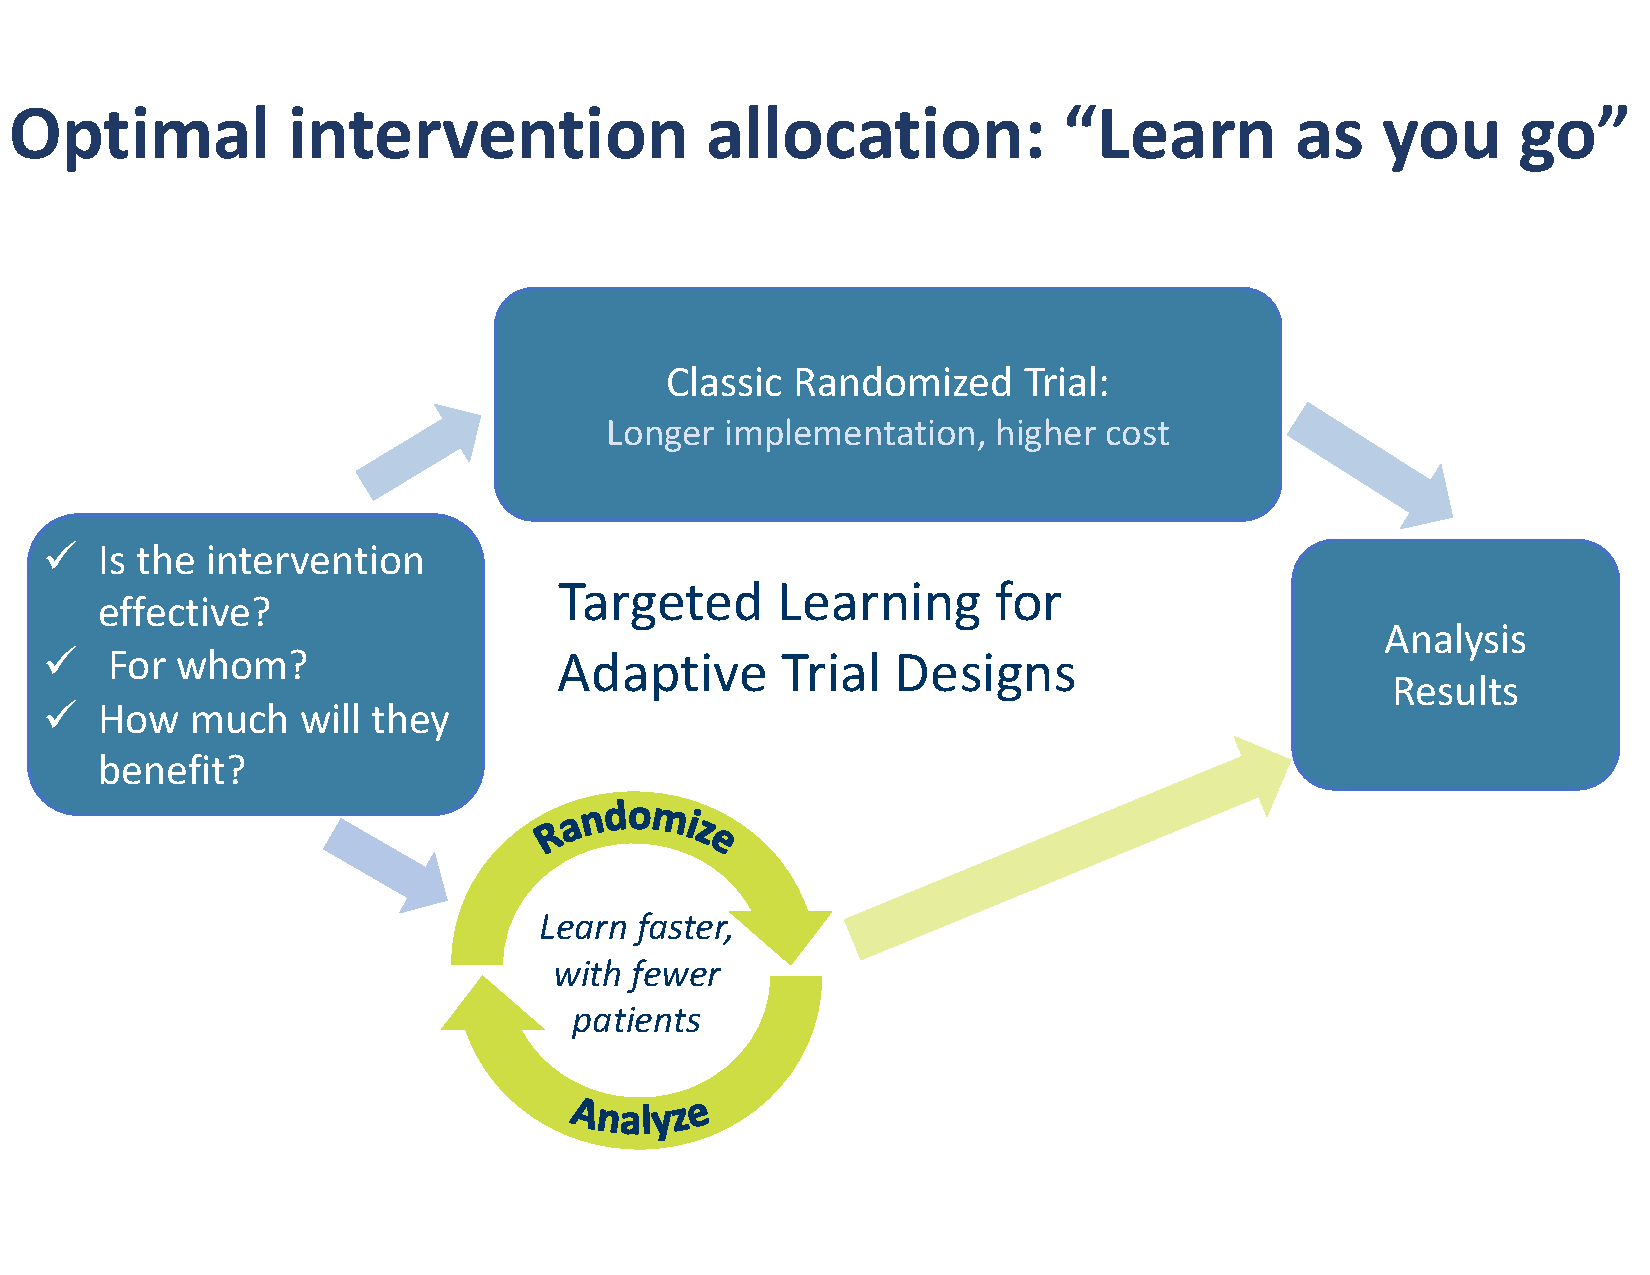
\includegraphics[scale=0.35]{learnasyougo_cropped.pdf}
\end{frame}


% \begin{frame}
% \frametitle{Adapting the randomization probabilities in a sequence of Sepsis RCTs}
% \begin{itemize}
%     \item We sequentially draw 8 blocks of 100 observations $(W_i,A_i,Y_i)$, $W$ including adrenal insufficiency (binary); serum levels.
%     \item At each block, we use {\bf super learning of optimal rule} and TMLE to estimate its {\bf counterfactual death rate}. 
%   % \item For the adaptive design we then set the randomization probabilities for next block accordingly, while balanced design keeps flipping coin when assigning treatment.
%     \item We report performance of the fixed balanced design and the adaptive design learning the optimal rule w.r.t.  {\bf percentage receiving optimal rule}; observed {\bf death rate}; {\bf coverage} of confidence  intervals.
%     \end{itemize}
%     \end{frame}

\begin{frame}
\frametitle{Balanced vs. adaptive sequential design}
\centering
\animategraphics[autoplay,loop,width=0.8\linewidth]{10}{Survival_PercentSamples/gganim_plot}{0001}{0100}
\end{frame}

\begin{frame}
\frametitle{Balanced vs. adaptive sequential design}
\vspace{-5pt}
\begin{figure}%
    \centering
    %\caption{Width of the Confidence Interval and Percent Death in Balanced and Adaptive Sequential Trial}%
    \subfloat{{\animategraphics[autoplay,loop,width=0.49\linewidth,height=0.49\linewidth]{10}{Survival_WidthCI/gganim_plot}{0001}{0100} }}%
    %\qquad
    \subfloat{{\animategraphics[autoplay,loop,width=0.49\linewidth,height=0.49\linewidth]{10}{Survival_MeanOutcome/gganim_plot}{0001}{0100} }}%
    %\label{fig:example}%
\end{figure}
\end{frame}


% \begin{frame}
% \frametitle{Convergence of adaptive randomization probabilities towards optimal rule}
% \vspace{5pt}
% \centering
% \begin{figure}%
% \includegraphics[scale=0.3]{design_convergence}
% \end{figure}
% \end{frame}


% \begin{frame}{TMLE-based statistical inference for performance under current best estimate of rule}
% \vspace{15pt}
%     \includegraphics[scale=0.3]{adaptive_design_inference}
% \end{frame}
% \subsection{Complex Observational Studies}

% \begin{frame}
% \frametitle{Longitudinal data structure}
% We observe $n$ i.i.d. copies of a longitudinal data structure
% \[
% O=(L(0),A(0),\ldots,L(K),A(K),Y=L(K+1)),\]
% where 
% \begin{itemize}
%     \item $A(t)$ denotes a discrete valued {\bf intervention node} whose effect we desire to evaluate
%     \item $L(t)$ is an {\bf intermediate covariate/outcome} realized in between intervention nodes $A(t-1)$ and $A(t)$, $t=0,\ldots,K$
%     \item $Y$ is the {\bf final outcome} of interest
% \end{itemize}    
% \end{frame}
% \begin{frame}
% \frametitle{Survival outcome example}
% \begin{eqnarray*}
% A(t)&=&(A_1(t),A_2(t))\\
% A_1(t)&=& \mbox{Indicator of being treated at time $t$}\\
% A_2(t)&=& \mbox{Indicator of being right-censored at time $t$}\\
% %\Delta&=&\mbox{Indicator of observing failure}\\
% Y(t)&=&\mbox{Indicator of observing a failure by time $t$}\\
% L(t)&=&\mbox{Vector of time-dependent measurements}\\
% Y(t)&\subset& L(t) \mbox{and  $Y=Y(K+1)$}.
% \end{eqnarray*}
% \end{frame}

% \begin{frame}
% \frametitle{Likelihood and statistical model}
% The probability distribution $P_0$ of $O$ can be factorized according to the time-ordering as 
% \begin{eqnarray*}
% p_0(O)&=&\prod_{t=0}^{K+1} p_0(L(t)\mid Pa(L(t)) ) \prod_{t=0}^K p_0(A(t)\mid Pa(A(t)) )\\
% &\equiv& \prod_{t=0}^{K+1}q_{0,L(t)}(O)\prod_{t=0}^K g_{0,A(t)}(O)\\
% &\equiv& q_0g_0,
% \end{eqnarray*}
% {\footnotesize
% where $Pa(L(t))\equiv (\bar{L}(t-1),\bar{A}(t-1))$ and $Pa(A(t))\equiv (\bar{L}(t),\bar{A}(t-1))$ denote the parents of  $L(t)$ and $A(t)$, respectively. 

% The $g_0$-factor represents the intervention mechanism.}

% \vspace{15pt}

% {\bf Statistical Model:}
% We make no assumptions on $q_0$, but could make assumptions on $g_0$.
% \end{frame}

% \begin{frame}
% \frametitle{Target estimand}
% \begin{itemize}
% \item $p^{g^*}_0=q_0(o)g^*(o)$ is the $G$-computation formula for the post-intervention distribution of $O$ under the stochastic intervention $g^*=\prod_{t=0}^K g^*_{A(t)}(O)$.

% \vspace{20pt}

% \item Target estimand $\Psi(P)=E_{P_{g^*}}Y$, i.e.,  mean outcome under $P_{g^*}$. 
% \end{itemize}
% \end{frame}

\section{Online Learning}

\begin{frame}
\frametitle{Online super learning in the ICU}

\begin{block}{\large{Adaptive algorithm}}
\begin{itemize}
\vspace{.15in}
\item Regularly updated with batches of new data
\vspace{.075in}
\item Learns from both
\begin{enumerate}
    \item within individual time series, and
    \vspace{.05in}
    \item across patients
\end{enumerate}
\vspace{.025in}
\item Uncertainty of forecasts assessed with prediction intervals
\vspace{.15in}
\end{itemize}
\end{block}

\end{frame}

\begin{frame}
\frametitle{15-minute ahead forecasts with prediction intervals for patient with hypotensive episodes}
% Individualized online super learner (iOSL) for real-time, personalized forecasting with inference 
\centering

\animategraphics[autoplay,loop,width=0.95\linewidth, controls=play]{3}{iOSL/plot}{002}{207}

\end{frame}


\section{Future of Targeted Learning}
\begin{frame}
\frametitle{Future of Targeted Learning}
\vspace{-20pt}
\begin{center}
  \includegraphics[width=1.05\textwidth]{future.pdf}
  \end{center}
\end{frame}

\end{document}


\end{document}
